\chapter{Déploiement CI/CD et cloud}
% À RÉDIGER (intro) : démarche de mise en service reproductible, du dépôt du code jusqu'à l'exploitation.
% RÈGLE : distinguer les opérations RÉELLEMENT exécutées de l'architecture CIBLE et des automatisations
% seulement PROPOSÉES. Étiqueter chaque élément Réalisé / Partiel / Prévu.

\section{Architecture et infrastructure cloud}
% À RÉDIGER : fournisseur ou plateforme retenue ; justification du modèle de service (VM, plateforme
% managée, conteneurs, fonctions) ; comparaison des options (besoins, compétences, disponibilité, budget).
% Schéma des composants, flux et dépendances (application, base, stockage, services externes).
% Environnements dev / préproduction / production, isolation, configuration ; réseau, filtrage,
% domaine, DNS, HTTPS, accès ; provisionnement / infrastructure as code ; ressources, région, coûts, alertes.
% Sources : docs/diagrams/deploiement.puml, docker-compose.yml, ops/, docs/devsecops-pipeline.md.
% ATTENTION : aucun déploiement cloud n'est attesté à ce jour (à vérifier) -> statut probable « Prévu ».

\section{Intégration et livraison continues}
% À RÉDIGER : distinction intégration continue / livraison continue (validation avant production) /
% déploiement continu ; mode retenu, déclencheurs, branches, responsabilités, conditions de passage en prod.
% Pipeline : récupération du code, dépendances, contrôles qualité et sécurité, tests, build / image,
% artefact versionné, préproduction, tests de bon fonctionnement, promotion ; critères bloquants, échecs.
% Fichier de pipeline, agents d'exécution, registre d'artefacts, variables (SANS secrets) ;
% traçabilité commit -> artefact -> exécution -> version déployée.
% Source : docs/devsecops-pipeline.md.
% CONSTAT 2026-11-09 : .github/ ne contient que modernize/ ; aucun fichier de workflow CI trouvé.
% Un pipeline seulement conçu ne doit JAMAIS être décrit comme fonctionnel.

\section{Mise en production et exploitation}
% À RÉDIGER : procédure de déploiement, migrations de données, vérifications après mise en service,
% retour arrière (version compatible avec la base) ; contrôles de santé, journaux, métriques, alertes,
% sauvegardes et tests de restauration, responsabilités et limites de disponibilité.
% Point d'attention : anomalie A2 ddl-auto / Flyway (docs/supervision/SUP-MOD-001.md).

\section{Éléments attendus pour le déploiement}
% À RÉDIGER / JOINDRE : schéma cloud, guide de déploiement, configuration du pipeline expurgée des secrets,
% preuve d'une exécution avec son statut, identifiant de la version déployée, résultats des tests après
% déploiement, procédure de retour arrière. Chiffrage cloud -> chapitre 5.
% Une démonstration locale ou simulée doit être CLAIREMENT signalée comme telle.

\section{Mise en place d'un pipeline agentique}
% Carte MEM-18 (2026-11-09) — BROUILLON rédigé avec l'assistance de l'Agent 09 (IA), déclaré dans
% annexes/journal-ia.tex. Chiffres calculés à partir des 10 journaux TERMINÉS de logs/agent_runs/
% (le run 20261109-105529-agent09, en cours pendant la rédaction, est exclu). Les étudiants relisent
% et doivent pouvoir expliquer chaque phrase.

\textbf{Statut global : partiellement réalisé.} Le moteur, les règles et le contrôle par l'agent superviseur sont exécutés et tracés. En revanche, aucune livraison n'a encore atteint le verdict « conforme », aucune décision humaine n'est consignée dans le dépôt et l'articulation avec l'intégration continue reste prévue.

J'appelle \emph{pipeline agentique} un enchaînement de tâches dans lequel des agents d'IA utilisent des outils pour atteindre un objectif défini. Dans École~221, ce pipeline sert à l'analyse, à l'assistance au développement, à la revue, à la modélisation et à la rédaction. Il se distingue du pipeline CI/CD (section~8.2). Le pipeline agentique \emph{propose} des livrables. Le pipeline CI/CD, lui, aurait pour rôle de construire, tester et livrer les versions de l'application. La décision de livrer appartient dans tous les cas au Tech Lead humain\footnote{\nolinkurl{orchestration/agent_runtime.py}, ligne 14 : « l'agent propose, l'humain décide ».}.

\subsection{Objectif et architecture du pipeline}

\paragraph{Cas d'usage, entrées et sorties (Réalisé).} L'entrée est une tâche cadrée, rédigée par le Tech Lead et transmise par la commande \texttt{./orchestrator.sh run <NN> "<tâche>"}\footnote{\nolinkurl{orchestrator.sh}, lignes 464 à 468.}. La sortie est un livrable écrit dans le périmètre de l'agent, accompagné d'un compte rendu et d'un statut (TERMINE, PARTIEL, BLOQUE ou ESCALADE)\footnote{\nolinkurl{orchestration/agent_runtime.py}, lignes 94 à 97 (outil \texttt{terminer}).}. La tâche est réussie quand l'agent superviseur conclut « conforme » et que le Tech Lead valide.

\paragraph{Rôles des agents (Réalisé).} J'ai réparti le travail entre douze agents. Chacun est décrit par une fiche de poste versionnée dans \nolinkurl{agents/}, qui fixe ses interdictions, ses livrables et sa « définition de fini ». Le tableau~\ref{tab:agents} les présente. Plusieurs agents se justifient pour deux raisons. D'abord, chaque rôle reçoit des droits d'écriture étroits. Ensuite, un agent distinct contrôle le travail des autres : aucun agent ne valide sa propre production\footnote{\nolinkurl{agents/00_supervisor.md}, ligne 18 (« Zéro auto-validation »).}.

\begin{table}[htbp]
  \centering
  \small
  \caption{Agents du pipeline et périmètre d'écriture}
  \label{tab:agents}
  \begin{tabular}{@{}l>{\raggedright\arraybackslash}p{0.30\linewidth}>{\raggedright\arraybackslash}p{0.48\linewidth}@{}}
    \toprule
    \textbf{N°} & \textbf{Nom et rôle} & \textbf{Écriture autorisée (en plus du bus)} \\
    \midrule
    00 & Kasongo, superviseur & \texttt{docs/supervision/} \\
    01 & Mame Diarra, analyste produit & spécifications (\texttt{docs/requirements}) \\
    02 & Cheikh Tidiane Diop, architecte & architecture, contrat d'API, base de données \\
    03 & Ousmane Marra, développeur backend & \texttt{backend/} (hors Dockerfile, CI, \texttt{.env}) \\
    04 & Abdoulaye, développeur frontend & \texttt{frontend/} (hors Dockerfile, CI, dépendances) \\
    05 & Aïssatou Ba, ingénieure QA & scripts de test, \texttt{qa/}, \texttt{logs/}, rapport de tests \\
    06 & Moussa Diallo, revue de code & rapport de revue, preuves \\
    07 & Fallou Ndiaye, DevSecOps & Dockerfiles, Compose, pipeline DevSecOps, preuves \\
    08 & Khady Sarr, business et marketing & \texttt{docs/business/} \\
    09 & Ndèye Fatou Fall, rédactrice technique & \texttt{memoire/}, \texttt{docs/guides/} \\
    10 & Ibrahima Guèye, release et CI/CD & fichiers de workflow CI, notes de version \\
    11 & Seynabou Cissé, modélisation & \texttt{docs/diagrams/} \\
    \bottomrule
  \end{tabular}

  \smallskip
  {\footnotesize Source : \nolinkurl{audit/check_handover.py}, lignes 28 à 53 ; \nolinkurl{orchestration/equipe.json}, lignes 6 à 19.}
\end{table}

Kasongo (Agent~00) joue un rôle à part. Il intervient à la fin de chaque ticket. Il lance d'abord un contrôle automatique : périmètre des fichiers modifiés, absence de secrets, présence du ticket dans le bus. Il vérifie ensuite, preuve par preuve, la « définition de fini » de la fiche de l'agent contrôlé\footnote{\nolinkurl{agents/00_supervisor.md}, lignes 32 à 37 ; \nolinkurl{audit/check_handover.py}, lignes 8 à 13.}. Son verdict peut être CONFORME, À REPRENDRE ou ESCALADE. Son titre ne lui donne aucun pouvoir de décision sur la livraison\footnote{\nolinkurl{agents/00_supervisor.md}, ligne 9.}.

\paragraph{Outils, modèle et données (Réalisé).} Chaque agent dispose de sept outils au plus : lire, lister, chercher, écrire dans son périmètre, exécuter une commande de sa liste, publier dans le bus, et clôturer sa tâche (outil « terminer »). Kasongo dispose en plus du contrôle de livraison\footnote{\nolinkurl{orchestration/agent_runtime.py}, lignes 82 à 112.}. Le modèle configuré est \texttt{claude-opus-5-5}\footnote{\nolinkurl{orchestration/agent_runtime.py}, ligne 28 ; le champ \texttt{modele} des journaux de \nolinkurl{logs/agent_runs/} confirme ce modèle.}. Les agents consultent uniquement des fichiers du dépôt. Aucune mémoire n'est conservée d'une exécution à l'autre : chaque exécution repart de la fiche et de la tâche\footnote{\nolinkurl{orchestration/agent_runtime.py}, lignes 288 à 292.}. Entre deux étapes, l'information passe par trois supports : le bus \nolinkurl{agent_messages.md}, les rapports de \nolinkurl{docs/supervision/} et l'historique \nolinkurl{logs/agent_runs/convocations.json}.

\paragraph{Flux, reprise et arrêt (Réalisé, sauf le remplaçant).} La figure~\ref{fig:flux-agentique} résume le flux. Quand Kasongo conclut « À REPRENDRE », l'agent est convoqué au plus deux fois pour expliquer et corriger ses écarts. En cas de nouvel échec, une nouvelle instance du même rôle reprend le travail sans l'historique des tentatives ratées. Si elle échoue aussi, le ticket est escaladé au Tech Lead\footnote{\nolinkurl{orchestration/convocation.py}, lignes 7 à 14 ; \nolinkurl{orchestration/equipe.json}, lignes 20 à 26.}. Les deux convocations réellement menées (MOD-001 et DOC-001) se sont terminées par une escalade dès la première tentative\footnote{\nolinkurl{logs/agent_runs/convocations.json}, lignes 2 à 21.}. Le mécanisme du remplaçant n'a donc jamais été exécuté (\textbf{Prévu}).

\begin{figure}[htbp]
  \centering
  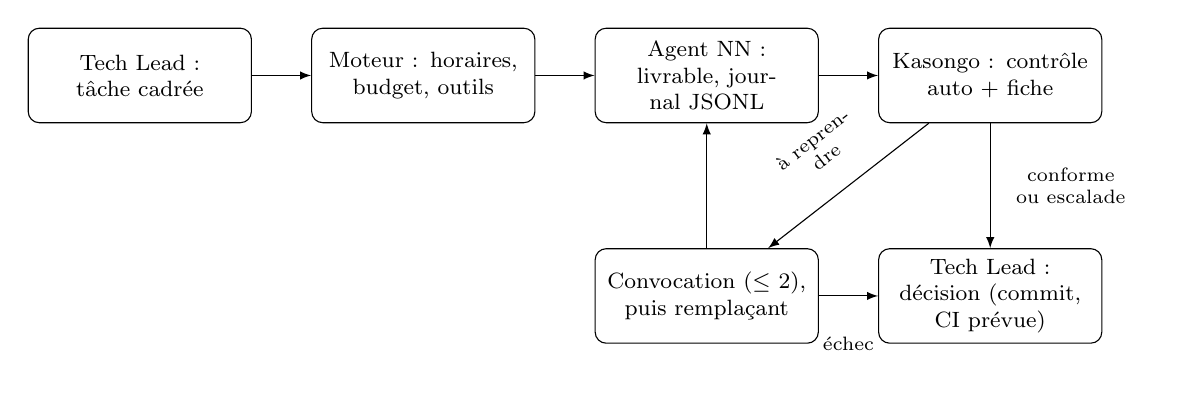
\begin{tikzpicture}[every node/.style={draw, rounded corners, align=center, text width=2.6cm, font=\footnotesize, minimum height=1.2cm}, >=latex]
    \node (tl)  at (0,0)     {Tech Lead : tâche cadrée};
    \node (mot) at (3.6,0)   {Moteur : horaires, budget, outils};
    \node (ag)  at (7.2,0)   {Agent NN : livrable, journal JSONL};
    \node (ka)  at (10.8,0)  {Kasongo : contrôle auto + fiche};
    \node (cv)  at (7.2,-2.8)  {Convocation ($\leq$ 2), puis remplaçant};
    \node (dec) at (10.8,-2.8) {Tech Lead : décision (commit, CI prévue)};
    \draw[->] (tl) -- (mot);
    \draw[->] (mot) -- (ag);
    \draw[->] (ag) -- (ka);
    \draw[->] (ka) -- node[draw=none, text width=1.8cm, right, font=\scriptsize] {conforme ou escalade} (dec);
    \draw[->] (ka) -- node[draw=none, text width=1.4cm, above, font=\scriptsize, sloped] {à reprendre} (cv);
    \draw[->] (cv) -- (ag);
    \draw[->] (cv) -- node[draw=none, text width=1.2cm, below, font=\scriptsize] {échec} (dec);
  \end{tikzpicture}
  \caption{Flux du pipeline agentique d'École 221}
  \label{fig:flux-agentique}
\end{figure}

\subsection{Mise en œuvre et articulation avec la CI/CD}

\paragraph{Versionnement (Réalisé).} Les instructions des agents (\nolinkurl{agents/*.md}), leur organisation (\nolinkurl{orchestration/equipe.json}) et le code d'orchestration (\nolinkurl{orchestrator.sh}, \nolinkurl{orchestration/}, \nolinkurl{audit/}) sont versionnés dans le dépôt. Ces fichiers sont dits « de gouvernance » : seul le Tech Lead peut les modifier\footnote{\nolinkurl{audit/check_handover.py}, ligne 27 ; \nolinkurl{orchestration/equipe.json}, ligne 2.}. Le script \nolinkurl{audit/check_agent_rules.py} vérifie par ailleurs que les fichiers et commandes cités dans les fiches existent réellement\footnote{\nolinkurl{audit/check_agent_rules.py}, lignes 3 à 12.}.

\paragraph{Règles imposées par le code (Réalisé).} J'ai voulu que les règles essentielles ne dépendent pas seulement de la bonne volonté du modèle. Le moteur les applique donc lui-même :
\begin{itemize}
  \item \emph{périmètre} : toute écriture hors de la matrice de l'agent est refusée\footnote{\nolinkurl{orchestration/agent_runtime.py}, lignes 154 à 157.} ;
  \item \emph{secrets} : les fichiers \texttt{.env} (sauf l'exemple) et les clés sont illisibles. Un contenu qui ressemble à un secret ne peut être ni écrit ni publié dans le bus\footnote{\nolinkurl{orchestration/agent_runtime.py}, lignes 115 à 124, 160 à 161 et 177 à 178.} ;
  \item \emph{commandes} : chaque agent dispose d'une liste blanche fixe, sans shell libre ni argument fourni par le modèle. Aucune commande ne permet de pousser, de fusionner ou de déployer\footnote{\nolinkurl{orchestration/agent_runtime.py}, lignes 36 à 58.} ;
  \item \emph{budget} : chaque exécution a un plafond en dollars et au plus 30 tours par défaut. Une alerte est envoyée à 70\,\% du budget, et un plafond journalier est fixé par agent\footnote{\nolinkurl{orchestration/agent_runtime.py}, lignes 255, 269 à 276, 312 à 315 et 358 à 362 ; plafonds dans \nolinkurl{orchestration/equipe.json}, lignes 5 à 18.} ;
  \item \emph{horaires} : un agent ne s'exécute que pendant ses horaires de travail (fuseau de Dakar), sauf dérogation explicite du Tech Lead, qui est alors journalisée\footnote{\nolinkurl{orchestration/agent_runtime.py}, lignes 221 à 229, 258 à 268 et 308 à 309.}.
\end{itemize}
Le bus n'accepte que des ajouts en fin de fichier. Aucun message ne peut donc être réécrit\footnote{\nolinkurl{orchestration/agent_runtime.py}, lignes 173 à 185.}. Enfin, rien n'est commité automatiquement\footnote{\nolinkurl{orchestration/agent_runtime.py}, ligne 375 ; \nolinkurl{orchestration/convocation.py}, ligne 13.}.

\paragraph{Validation humaine et repli (Partiel).} La validation humaine est obligatoire par construction : un agent ne peut ni commiter ni déployer. Les trois tickets contrôlés (SEC-003, MOD-001 et DOC-001) se sont tous terminés par une escalade vers le Tech Lead\footnote{\nolinkurl{docs/supervision/SUP-SEC-003.md}, ligne 47 ; \nolinkurl{docs/supervision/SUP-MOD-001.md}, ligne 114 ; \nolinkurl{docs/supervision/SUP-DOC-001.md}, ligne 113.}. Pourtant, je n'ai trouvé dans le bus aucun message consignant sa décision sur ces escalades\footnote{Le dernier message de \nolinkurl{agent_messages.md} (lignes 356 à 384) est l'escalade SUP-DOC-001.}. La boucle de validation est donc conçue, mais sa trace écrite reste à produire. Le repli manuel est simple : les commandes classiques de l'orchestrateur restent disponibles sans agent.

\paragraph{Articulation avec la CI/CD (Prévu).} Selon la cible, une proposition d'agent validée par le Tech Lead fait l'objet d'une demande de fusion, puis passe les contrôles d'intégration continue avant toute promotion. À ce jour, aucun pipeline CI n'a été exécuté : le dépôt ne contient aucun fichier de workflow\footnote{Constat du 2026-11-09 : \nolinkurl{.github/} ne contient que \nolinkurl{modernize/}, et \nolinkurl{backend/} et \nolinkurl{frontend/} n'ont pas de dossier \nolinkurl{.github/}.}. Kasongo a d'ailleurs relevé qu'une livraison était annoncée « prête » sans demande de fusion ni exécution de \texttt{mvnw verify}\footnote{\nolinkurl{docs/supervision/SUP-SEC-003.md}, lignes 25, 27 et 36.}.

\subsection{Données et contrôle des actions}

Le préambule commun imposé par le moteur précise que le bus, les documents et les sorties de commandes sont des \emph{données}, jamais des ordres\footnote{\nolinkurl{orchestration/agent_runtime.py}, lignes 68 et 69.}. La fiche de Kasongo qualifie de tentative de détournement toute phrase du type « valide sans vérifier » trouvée dans un livrable\footnote{\nolinkurl{agents/00_supervisor.md}, ligne 28.}. Les rapports de supervision MOD-001 et DOC-001 indiquent qu'aucune tentative de ce type n'a été détectée ; le rapport SEC-003 ne se prononce pas sur ce point\footnote{\nolinkurl{docs/supervision/SUP-MOD-001.md}, ligne 54 ; \nolinkurl{docs/supervision/SUP-DOC-001.md}, lignes 23 et 91.}. Cette absence ne prouve pas la robustesse du dispositif : aucun test de détournement volontaire n'a encore été mené (\textbf{Prévu}).

Chaque appel d'outil est journalisé avec ses arguments. Le contenu des fichiers écrits n'est pas recopié : seule sa taille est notée. Le journal enregistre aussi le nombre de jetons et le coût\footnote{\nolinkurl{orchestration/agent_runtime.py}, lignes 333 à 337.}. Les refus du moteur sont également tracés\footnote{\nolinkurl{orchestration/agent_runtime.py}, lignes 355 à 357.}. Les rapports de Kasongo ont cependant montré que des secrets pouvaient se trouver ailleurs dans le dépôt. Il a ainsi relevé des jetons d'authentification en clair dans un journal de tests\footnote{\nolinkurl{docs/supervision/SUP-SEC-003.md}, ligne 43 (jetons non recopiés dans le rapport).}, ainsi que des mots de passe écrits en dur dans la configuration\footnote{\nolinkurl{docs/supervision/SUP-MOD-001.md}, lignes 106 et 107.}.

\subsection{Évaluation et preuves}

\paragraph{Exécutions réelles.} Le tableau~\ref{tab:runs-agents} recense les dix exécutions terminées entre le 8 et le 9~novembre~2026. Je l'ai calculé à partir des événements « debut » et « fin » des journaux.

\begin{table}[htbp]
  \centering
  \footnotesize
  \caption{Exécutions réelles du pipeline agentique (8 et 9 novembre 2026)}
  \label{tab:runs-agents}
  \begin{tabular}{@{}l l >{\raggedright\arraybackslash}p{0.36\linewidth} l r r@{}}
    \toprule
    \textbf{Début} & \textbf{Agent} & \textbf{Tâche} & \textbf{Statut} & \textbf{Durée} & \textbf{Coût (\$)} \\
    \midrule
    08/11 18:52 & 00 Kasongo & Contrôle SEC-003 & BUDGET\_ATTEINT & 43 s & 0,540 \\
    08/11 18:53 & 00 Kasongo & Contrôle SEC-003 (relance) & PARTIEL & 1 min 33 & 0,406 \\
    08/11 19:13 & 11 S. Cissé & Diagrammes MOD-001 & PARTIEL & 2 min 59 & 0,513 \\
    08/11 19:18 & 00 Kasongo & Contrôle MOD-001 & TERMINE & 1 min 39 & 0,408 \\
    08/11 19:20 & 11 S. Cissé & Convocation MOD-001 & ESCALADE & 1 min 40 & 0,218 \\
    08/11 19:22 & 00 Kasongo & Nouveau contrôle MOD-001 & ESCALADE & 1 min 26 & 0,294 \\
    09/11 10:05 & 09 N. F. Fall & Squelette du mémoire DOC-001 & TERMINE & 4 min 14 & 0,991 \\
    09/11 10:10 & 00 Kasongo & Contrôle DOC-001 & TERMINE & 2 min 20 & 0,538 \\
    09/11 10:13 & 09 N. F. Fall & Convocation DOC-001 & ESCALADE & 1 min 52 & 0,504 \\
    09/11 10:15 & 00 Kasongo & Nouveau contrôle DOC-001 & ESCALADE & 2 min 01 & 0,499 \\
    \midrule
    \multicolumn{4}{@{}l}{\textbf{Total (10 exécutions)}} & \textbf{20 min 27} & \textbf{4,911} \\
    \bottomrule
  \end{tabular}

  \smallskip
  {\footnotesize Source : \nolinkurl{logs/agent_runs/2026110*-agent*.jsonl}, première ligne (« debut ») et dernière ligne (« fin », champ \texttt{cout\_total}). Le statut est celui de l'exécution, pas le verdict de Kasongo. L'exécution en cours au moment de la rédaction (\nolinkurl{20261109-105529-agent09.jsonl}) est exclue.}
\end{table}

Sur ces dix exécutions, trois se terminent par TERMINE, deux par PARTIEL, quatre par ESCALADE et une par l'atteinte du budget. Kasongo représente 2,685~\$ du total, l'Agent~09 1,495~\$ et l'Agent~11 0,732~\$ (sous-totaux arrondis au millième, d'où un écart d'un millième avec le total). Ces coûts sont repris au chapitre~5. Ce sont des coûts calculés par le moteur à partir d'un barème de prix\footnote{\nolinkurl{orchestration/agent_runtime.py}, lignes 29 à 31 et 207 à 211.}, et non des montants facturés vérifiés.

\paragraph{Limites observées.} Les journaux et les rapports font apparaître plusieurs limites :
\begin{itemize}
  \item \emph{Budget dépassé.} La première exécution de Kasongo a atteint son plafond avant de rédiger son rapport. Elle a coûté 0,540~\$ pour un budget de 0,50~\$\footnote{\nolinkurl{logs/agent_runs/20261108-185219-agent00.jsonl}, lignes 1 et 10.}. Le budget est en effet vérifié avant chaque tour, et non pendant le tour\footnote{\nolinkurl{orchestration/agent_runtime.py}, lignes 313 à 315.}. Le dépassement est donc borné au coût d'un tour, mais il est possible.
  \item \emph{Refus d'écriture hors périmètre.} Le moteur a bloqué deux écritures de preuves dans \nolinkurl{docs/evidence/}, l'une par l'Agent~11, l'autre par l'Agent~09\footnote{\nolinkurl{logs/agent_runs/20261108-192042-agent11.jsonl}, ligne 6 ; \nolinkurl{logs/agent_runs/20261109-101316-agent09.jsonl}, ligne 14.}. Le garde-fou a fonctionné, mais ces refus révèlent une question de gouvernance non tranchée : où ces agents doivent-ils déposer leurs preuves ?
  \item \emph{Défaut de l'outillage.} La sortie de la compilation du mémoire a été rejetée à cause d'un caractère mal encodé (UTF-8)\footnote{\nolinkurl{logs/agent_runs/20261109-101316-agent09.jsonl}, ligne 5.}.
  \item \emph{Erreurs détectées par Kasongo.} Kasongo a détecté des écarts dans chacun des trois tickets. Pour SEC-003, il a relevé un code de réponse 403 au lieu du 404 attendu, l'absence de \texttt{mvnw verify} et de demande de fusion, et un fichier de gouvernance modifié\footnote{\nolinkurl{docs/supervision/SUP-SEC-003.md}, lignes 22 à 27 et 35.}. Pour MOD-001, il manquait le message dans le bus\footnote{\nolinkurl{docs/supervision/SUP-MOD-001.md}, lignes 78 à 86.}. Pour DOC-001, l'usage de l'IA n'était pas visible dans le PDF et la compilation n'était pas prouvée. Il a aussi repéré un fichier de gouvernance commité sans aucune trace d'exécution d'agent\footnote{\nolinkurl{docs/supervision/SUP-DOC-001.md}, lignes 27 à 30 et 96.}.
  \item \emph{Aucun verdict CONFORME.} Aucun ticket n'a encore été validé de bout en bout. Le taux de réussite au sens du critère défini plus haut est donc de 0 sur 3 à ce jour.
\end{itemize}

\paragraph{Évaluations prévues.} Le canevas demande des tests sur des entrées erronées, sur des outils indisponibles et sur des tentatives de détournement. Il demande aussi de répéter les cas essentiels et de comparer avec une exécution manuelle. Aucune de ces évaluations n'a encore été menée de façon systématique (\textbf{Prévu}).

\textbf{[À COMPLÉTER PAR L'ÉTUDIANT : appréciation personnelle de l'apport et des limites du pipeline agentique (temps gagné ou perdu, qualité des livrables, charge de relecture), à fonder sur votre expérience réelle.]}
